\title{Supplementary material}
\author{}
\date{}

\begin{document}
\maketitle

In order to show how we implemented our framework and how model
components are translated into selection and drift dynamics we performed
simulations as described below. Our goal is to address main criticisms
of our framework being: (1) Are fixed and random effects actually
capturing selection and drift dynamics? (2) Are random effects only
capturing drift dynamics or uninformed species traits are inflating
random effects?

\subsection*{Material and Methods}\label{material-and-methods}

We use simulated communities based on selection and drift dynamics in
order to show how fixed and random effects capture different ecological
processes. Also, we use traits with strong and weak correlations to
species abundance in order to show how fixed and random effects capture
drift dynamics when traits are uninformative. Therefore, we simulate
stochastic and deterministic meta-communities and use strong or weak
traits in model selection.

We simulate meta-communities with the same data structure as our
abundance data of ferns in three mountain chains in southern Brazil.
Then, we make Poisson of communities and use samples from the
metacommunities in our model selection framework.

We analyze into three scenarios:

\begin{itemize}
\tightlist
\item
  Deterministic community with traits strongly correlated with species abundance from Poisson sample
\item
  Deterministic community with traits poorly correlated with species abundance from Poisson sample
\item
  Stochastic community with traits strongly correlated with species abundance from Poisson sample
\end{itemize}

\subsubsection*{Building simulated
communities}\label{building-simulated-communities}

We used the R
\href{package MCSIM}{http://rstudio-pubs-static.s3.amazonaws.com/159425_80725873417e42fdb13821c10a198281.html} from Eric Sokol to create simulations of metacommunities to test
assumptions about their underlying processes underlying (Sokol et
al.~2015). To replicate a data set analogous to our data all
metacommunities were composed by 30 sites in three regions with 153
species. We fixed the total number of individuals in the metacommunity
as 1000000 and migration parameter 0.5. Deterministic communities were
modelled based on an environmental gradient that weights the selection
of species from the species pool based on their traits. In addition,
deterministic communities exhibit a flat dispersal kernel. For
deterministic communities with strong traits, traits are highly
correlated with the environmental gradient. In, stochastic communities
species are also selected based on the environmental gradient, however
the standard deviation from the mean response to the gradient is
incredible high. Also, stochastic communities exhibit a dispersal
kernel of 200. For each scenario we generated 100 communities that were
then sampled with sampling effort of 20000 individuals. Our objective
here is to generate a scenario in which data is sampled from a Poisson
distribution, representing the structure of species abundance data

\subsubsection*{Fitting models to simulated
data}\label{fitting-models-to-simulated-data}

We used our framework to fit models for each community in the three
scenarios. We then calculated the proportion of the models with
\(\Delta{AIC} < 2\) belonging to each of our hypotheses and the adjusted
\(R^{2}\). We depicted all best models in terms of their adjusted
\(R^{2}\). Adjusted \(R^{2}\), as they measure the relative importance
of fixed and random effects in the model, are used here a proxy of
correspondence of community processes to terms in the model. We adapted
scripts from Johnson (2014) to calculate marginal and conditional
\(R^{2}\) of each models, and also the enhanced agreement repeatibility
(Stofel et al 2107), or the ratio of the intra-class variance for a
given random factor and the total variance estimated by the models,
including fixed-effect variances. These functions are available in the
script `functions.R' but applies only to models within our framework.
For generic functions please see packages (rptR and MuMIn).

% paragrafo resultados

\begin{table}[!ht]

\caption{\label{tab:table-prop}Proportion of models with {$\Delta$} AIC {$<$}  2 at each scenario.}
\centering
\begin{tabular}[t]{p{3cm}p{2.5cm}p{2.5cm}p{2.5cm}p{2.5cm}p{2.5cm}p{2.5cm}}
\toprule
\textbf{Scenario} & \textbf{Trait-mediated Selection} \& \textbf{Drift} & \textbf{Selection \& Drift} & \textbf{Trait-mediated Selection} & \textbf{Selection \& Drift} & \textbf{Idyosyncratic}\\
\hline
Deterministic with right traits & 1.00 & 0.00 & 0 & 0.00 & 0 & 0\\
Deterministic with wrong traits & 0.00 & 0.82 & 0 & 0.18 & 0 & 0\\
Stochastic with right traits & 0.02 & 0.00 & 0 & 0.00 & 1 & 0\\
\bottomrule
\end{tabular}
\end{table}

\begin{figure}
\centering
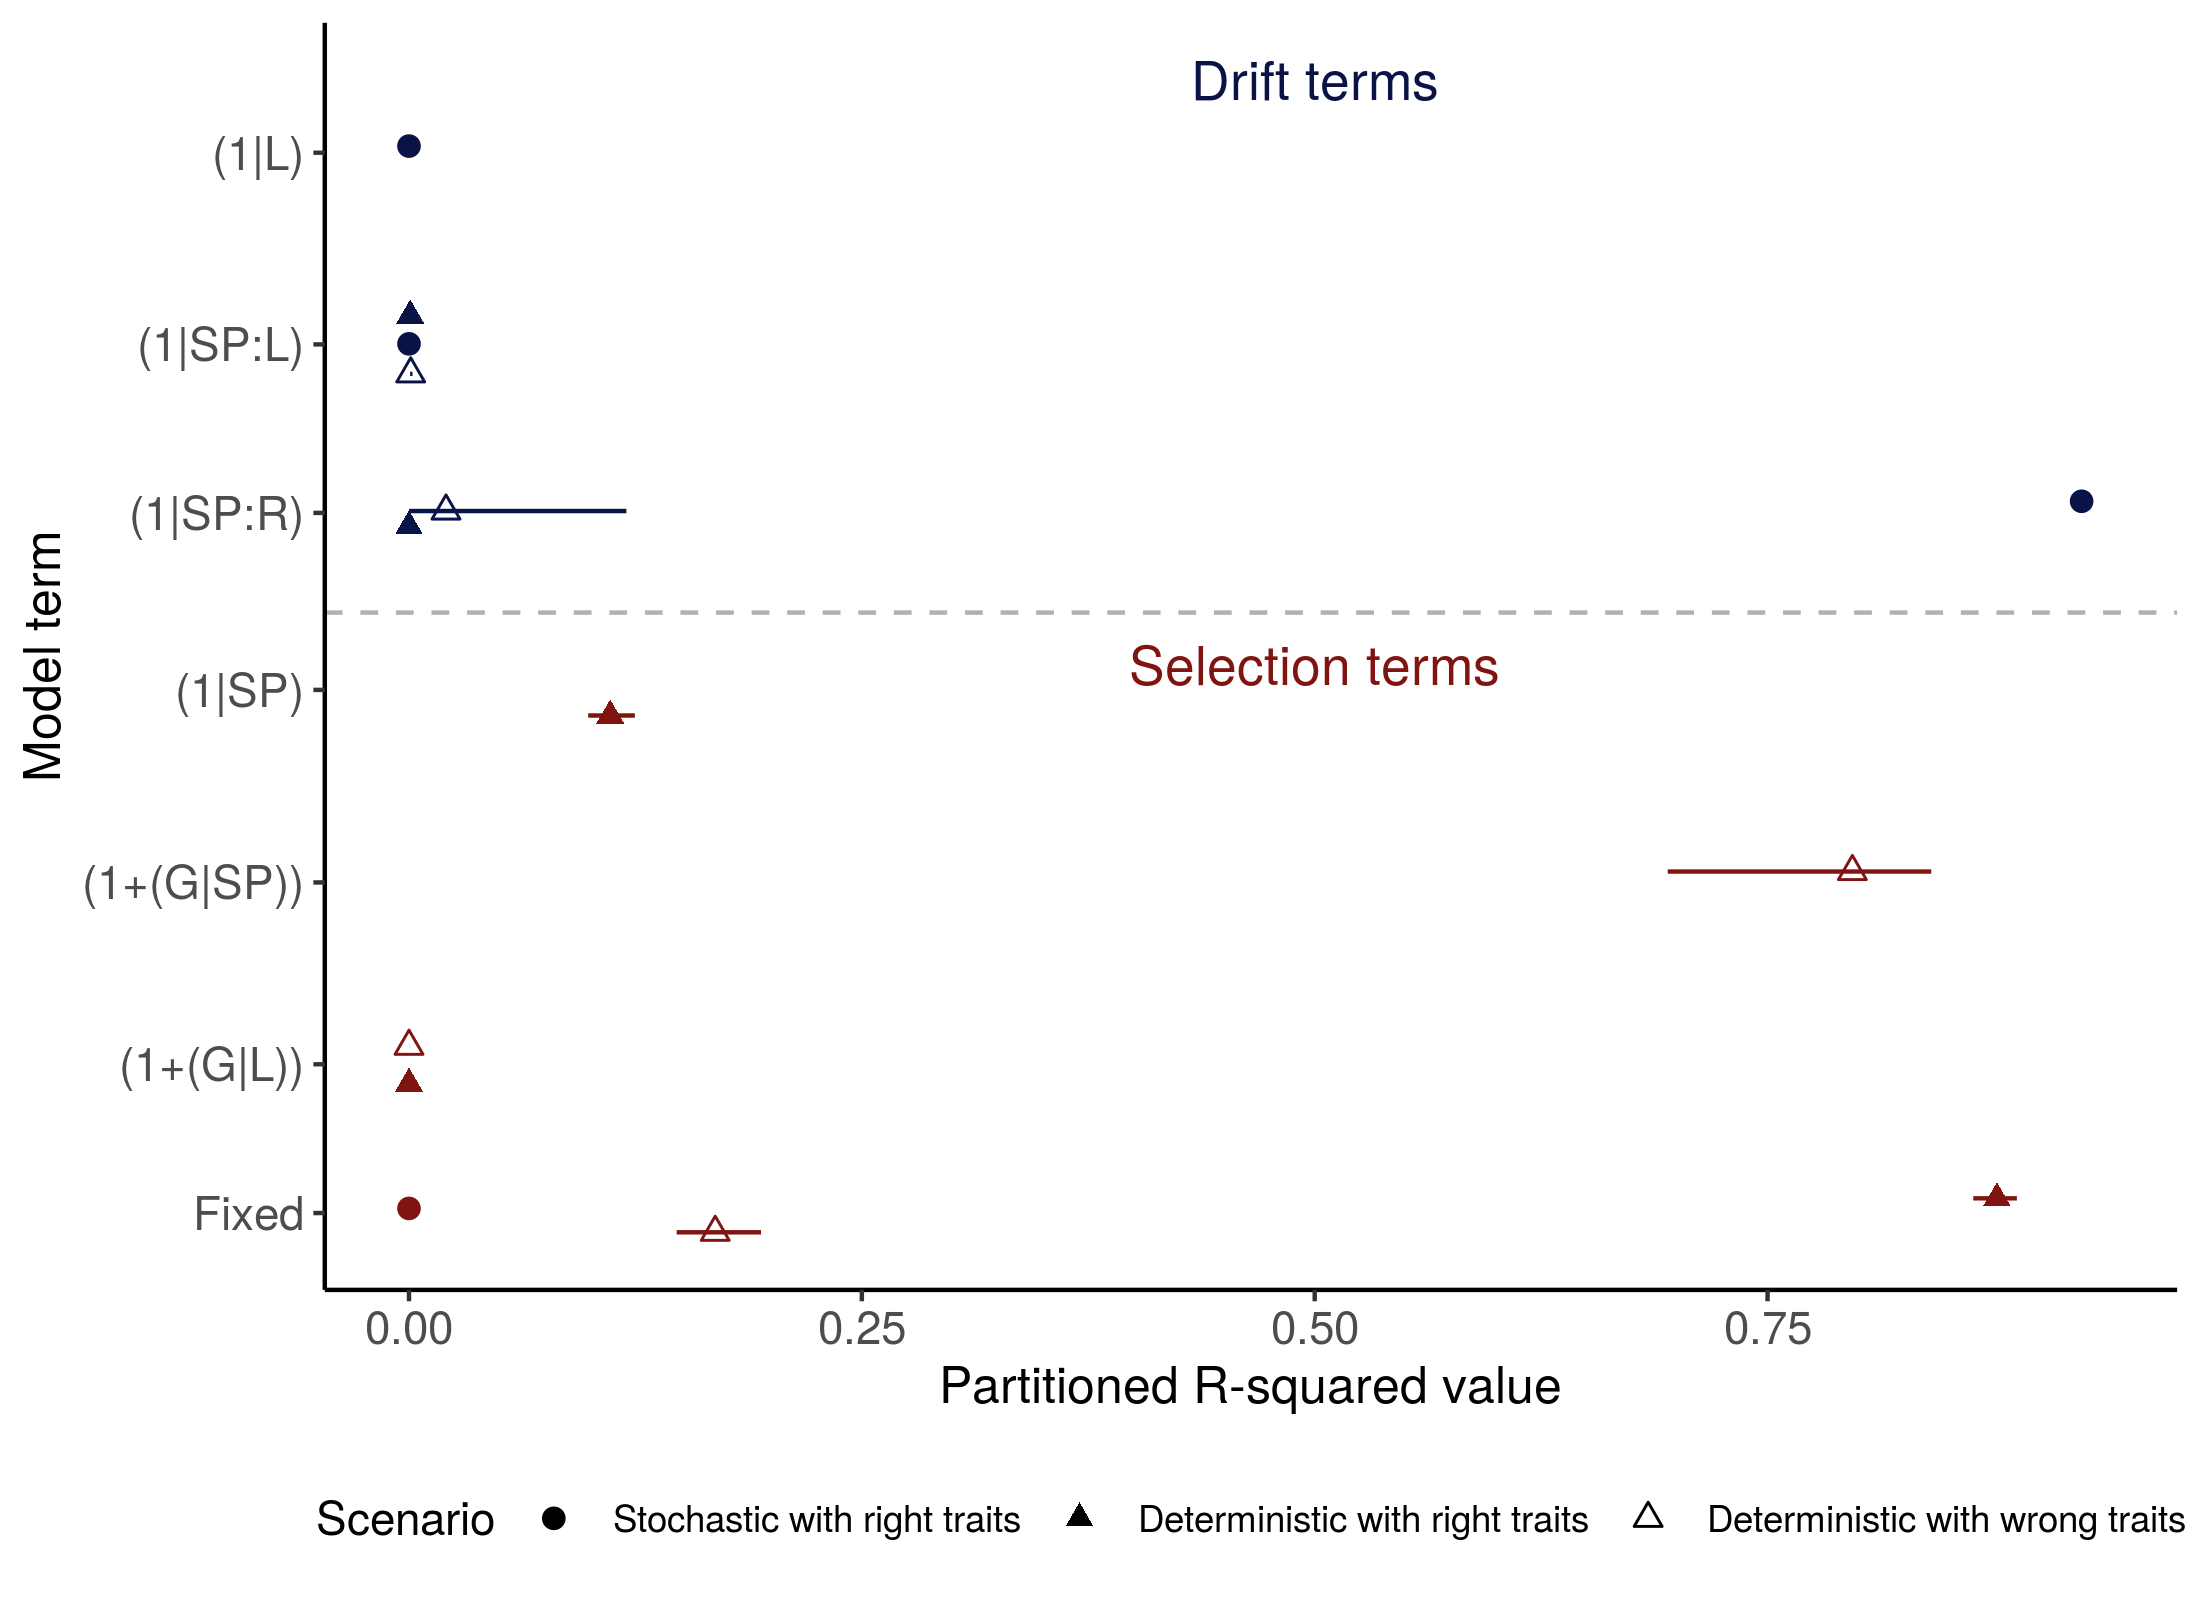
\includegraphics[scale=.9]{fig/S1.png}
\caption{Figure S1.}
\end{figure}

\end{document}
